\documentclass{book}
\usepackage[utf8]{inputenc}
\usepackage{amsfonts, amsmath, amssymb}
\usepackage{hyperref}
\usepackage{pgfplots}
\usepackage{asymptote}
\pgfplotsset{compat=1.18, width=10cm}
\usepackage[left=2cm,right=2cm,top=1cm,bottom=1.6cm]{geometry}
\usepackage{float}
\usetikzlibrary{shapes.misc}

\begin{document}
\section{Introduction}
The expression $f(x)=a_{0}x^{n}+a_{1}x^{n-1}+\ldots+a_{n-1}x+a_n$\\
where $\{a_i\}_{i=0}^{n}$ are constants and $a_0\neq0$ and $n\in\mathbb{Z}^{+}$ , is called a \textit{polynomial in }$x$\textit{ of degree }$n$. The polynomial $f(x)=0$ is called an \textit{algebraic equation of degree }$n$. If $f(x)$ contains some other function like trigonometric, logarithmic, exponential, etc. then $f(x)=0$ is said to be a \textit{transcendental equation}
\begin{asy}
   /* Geogebra to Asymptote conversion, documentation at artofproblemsolving.com/Wiki go to User:Azjps/geogebra */
import graph; size(22.9cm); 
real labelscalefactor = 0.5; /* changes label-to-point distance */
pen dps = linewidth(0.7) + fontsize(10); defaultpen(dps); /* default pen style */ 
pen dotstyle = black; /* point style */ 
real xmin = -6.48, xmax = 16.42, ymin = -3.6, ymax = 8.96;  /* image dimensions */
pen zzttqq = rgb(0.6,0.2,0.); pen qqwuqq = rgb(0.,0.39215686274509803,0.); pen cqcqcq = rgb(0.7529411764705882,0.7529411764705882,0.7529411764705882); pen svsvsv = rgb(0.1450980392156863,0.1450980392156863,0.1450980392156863); 

draw((3.68,3.78)--(7.44,1.68)--(3.02,0.66)--cycle, linewidth(2.) + zzttqq); 
draw((-1.54,3.44)--(2.42,2.62)--(4.34,4.68)--cycle, linewidth(2.) + zzttqq); 
 /* draw grid of horizontal/vertical lines */
pen gridstyle = linewidth(0.7) + cqcqcq; real gridx = 1., gridy = 1.; /* grid intervals */
for(real i = ceil(xmin/gridx)*gridx; i <= floor(xmax/gridx)*gridx; i += gridx)
 draw((i,ymin)--(i,ymax), gridstyle);
for(real i = ceil(ymin/gridy)*gridy; i <= floor(ymax/gridy)*gridy; i += gridy)
 draw((xmin,i)--(xmax,i), gridstyle);
 /* end grid */ 

Label laxis; laxis.p = fontsize(10); 
xaxis(xmin, xmax,defaultpen+svsvsv, Ticks(laxis, Step = 1., Size = 2, NoZero),EndArrow(6), above = true); 
yaxis(ymin, ymax,defaultpen+svsvsv, Ticks(laxis, Step = 1., Size = 2, NoZero),EndArrow(6), above = true); /* draws axes; NoZero hides '0' label */ 
 /* draw figures */
draw((3.68,3.78)--(7.44,1.68), linewidth(2.) + zzttqq); 
draw((7.44,1.68)--(3.02,0.66), linewidth(2.) + zzttqq); 
draw((3.02,0.66)--(3.68,3.78), linewidth(2.) + zzttqq); 
draw((-1.54,3.44)--(2.42,2.62), linewidth(2.) + zzttqq); 
draw((2.42,2.62)--(4.34,4.68), linewidth(2.) + zzttqq); 
draw((4.34,4.68)--(-1.54,3.44), linewidth(2.) + zzttqq); 
real f1 (real x) {return x^(2)+2+5*x^(4);} 
draw(graph(f1,-6.47,16.41), linewidth(2.) + qqwuqq); 
 /* dots and labels */
dot((3.68,3.78),dotstyle); 
label("$A$", (3.76,3.98), NE * labelscalefactor); 
dot((7.44,1.68),dotstyle); 
label("$B$", (7.52,1.88), NE * labelscalefactor); 
dot((3.02,0.66),dotstyle); 
label("$C$", (3.1,0.86), NE * labelscalefactor); 
label("$c$", (5.4,2.46), NE * labelscalefactor,zzttqq); 
label("$a$", (5.14,1.5), NE * labelscalefactor,zzttqq); 
label("$b$", (3.66,2.16), NE * labelscalefactor,zzttqq); 
dot((-1.54,3.44),dotstyle); 
label("$D$", (-1.46,3.64), NE * labelscalefactor); 
dot((2.42,2.62),dotstyle); 
label("$E$", (2.5,2.82), NE * labelscalefactor); 
dot((4.34,4.68),dotstyle); 
label("$F$", (4.42,4.88), NE * labelscalefactor); 
label("$f$", (0.36,2.72), NE * labelscalefactor,zzttqq); 
label("$d$", (3.6,3.44), NE * labelscalefactor,zzttqq); 
label("$e$", (1.32,4.38), NE * labelscalefactor,zzttqq); 
label("$g$", (-1.06,8.48), NE * labelscalefactor,qqwuqq); 
clip((xmin,ymin)--(xmin,ymax)--(xmax,ymax)--(xmax,ymin)--cycle); 
 /* end of picture */
\end{asy}
\begin{equation}
\text{The value of } x \text{ for which }f(x)=0, 	\label{eq:1.1}
\end{equation}
is called its \textit{root or solution}. Geometrically, a root of $(\ref{eq:1.1})$ is that value of $x$ where the graph of $y=f(x)$ crosses the x-axis. We often come across problems in deflection of beams, electrical circuit and mechanical vibration which depend upon the \textit{solution} of these equations. Hence, they are of great importance in the field of Applied as well as Pure Mathematics.

\section{General Properties}
\begin{enumerate}
\item If $\alpha$ is a \textit{root of the polynomial equation }$f(x)=0$, then the polynomial $f(x)$ is \textit{exactly divisible by }$x-\alpha$ and conversely.\\
\textbf{For example:} $x=3$ is a solution of $x^{4}-6x^{2}-8x-3=0$ since it satisfies the equation.\\
$\therefore$ $(x-3)$ is a factor of $x^{4}-6x^{2}-8x-3=0$

\item Every \textit{algebraic equation of degree }$n$\textit{ has }$n$\textit{ roots (real or imaginary)}.\\
Conversely, if $\{\alpha_{i}\}_{i=1}^{n}=\{\alpha_{1}, \alpha_{2}, \alpha_{3}\ldots\alpha_{n}\}$ are the roots of $nth$ \textit{degree polynomial }${f(x)=0}$, then \begin{equation}f(x)=A\prod_{i=1}^{n}(x-\alpha_{i})=A(x-\alpha_{1})(x-\alpha_2)(x-\alpha_3)\cdots(x-\alpha_{n})\label{eq:1.2}\end{equation}where $A$ is a constant.

$\textbf{Obs1. }\boxed{\text{a polynomial of }n\text{ degree has more than }n\text{ solutions, then it must be identically zero}}$

\item\textbf{Intermediate Value Property:} If $f(a)$ and $f(b)$ have different signs, then the equation $f(x)=0$ must have an \textit{odd number of roots} between $x=a$ and $x=b$.

Similarly, if $f(a)$ and $f(b)$ have same signs, then the equation $f(x)=0$ must have an \textit{even number of roots} between $x=a$ and $x=b$
\\
\begin{figure}[H]
\centering
\begin{tikzpicture}
\begin{axis}[
axis lines=middle,
ymin=-10,
ymax=25,
domain=-3.5:3,
xmajorgrids=false,
ymajorgrids=false,
xtick={-1.5, 1.5, 0.5},
xticklabels={$x=a$, $x=b$, $x=\alpha$},
ytick={},
yticklabels={},
xticklabel style={anchor=south west},
grid style=dashed
]
\addplot[color=red, samples=200]{2*x^3 - 13*x + x^2 + 6}; 

\draw[gray, dashed] (-1.5, 0) -- (-1.5, 21);
\draw[gray, dashed] (1.5, 0) -- (1.5, -4.5);
\filldraw[black] (-1.5, 21) circle[radius=2pt];
\filldraw[black] (1.5, -4.5) circle[radius=2pt];
\draw (-1.8, 10) node []{$f(a)$};
\draw (1.5, -6) node []{$f(b)$};
\filldraw[black] (1/2, 0) circle [radius=2pt];

\end{axis}
\end{tikzpicture}
\caption{}
\end{figure}
\pagebreak
\textbf{For different signs: }Since every polynomial function is \textit{continuous}, so while $x$ changes from $a$ to $b$, it must pass through all values from $f(a)$ to $f(b)$. Its trivial to notice that the function must end up in the opposite part of the \textit{x axis} from where it started if $f(a)$ and $f(b)$ have opposite signs .\\Also, $f(b)$ is at the other side of \textit{x axis}, the function MUST pass through the axis atleast once. After passing through the axis once, it reaches the other side of axis. Now, the function can either stay at the same side and reach $f(b)$. Or else, it will pass through the axis once again after which it comes back to the partition of axis it initially came from. So it has to cross the axis once again in order to reach the other part of axis.\\Observe how the function crosses the axis either \textit{once or }$3$\textit{ or }$5 \ldots$\textit{ times}.

\textbf{For same signs:} $f(a)$ and $f(b)$ are now at the same side of $x\ axis$. So the function must return to its initial zone. In the light of above point, its clear to see that the function must pass through $x\ axis\ even$ number of times and hence have even number of $solutions$.

\item \textit{In an equation with real coefficients, the imaginary roots occurs in conjugate pair. i.e,} if $\alpha+i\beta$ is a root of $f(x)=0$ where all the coefficients are \textit{real number}. Then $\alpha-i\beta$ must also be a root of the equation.\\Where $(\alpha, \beta)\in\mathbb{R}^{2}$ and $i=\sqrt{-1}$.

\textbf{Obs2.} $\boxed{\text{Every equation of an odd degree has atleast }1\text{ real root}}$

\item \textit{In an equation with rational coefficients, the irrational roots occurs in conjugate surds pair. i.e,} if $\alpha+\sqrt\beta$ is a root of $f(x)=0$ where all the coefficients are \textit{rational numbers}. Then $\alpha-\sqrt\beta$ must also be a root of the equation.\\Where $(\alpha, \beta)\in\mathbb{Z}^{2}$.

\item \textbf{Descarte's rule of signs:} The maximum number of \textit{positive roots} of $f(x)=0$ is equal to the \textit{number of sign changes of coefficients in }$f(x)$.\\And the maximum number of \textit{negative roots} of $f(x)=0$ is equal to the \textit{numbers of sign changes of coefficients} $in\ f(-x)$
\\
\textbf{Example:} consider $f(x)=2x^{7}-x^{5}+4x^{3}-5=0$\\
Sign of coefficients of $f(x)$:
\begin{center}
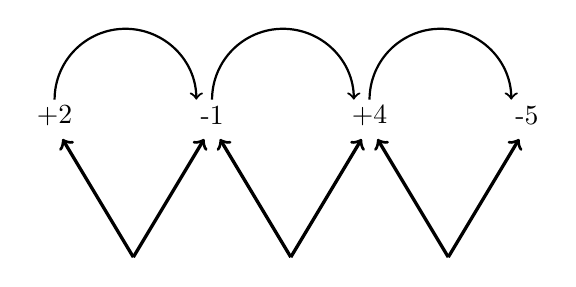
\begin{tikzpicture}[]
%\draw (-3, 0) -- (3, 0);
%\draw (0, 2.5) -- (0, -1.5);
%\draw[help lines] (-3, -1.4) grid (3, 1.4);
\draw [<-,very thick] (-2.9, .5) -- (-2, -1);
\draw [<-,very thick] (-1.1, .5) -- (-2, -1);
\draw [<-,very thick] (-.9, .5) -- (0, -1);
\draw [<-,very thick] (.9, .5) -- (0, -1);
\draw [<-,very thick] (1.1, .5) -- (2, -1);
\draw [<-,very thick] (2.9, .5) -- (2, -1);
\draw [->, thick] (-3, 1) arc [start angle = 180, end angle=0, radius=.9];
\draw [->, thick] (-1, 1) arc [start angle = 180, end angle = 0, radius=0.9];
\draw [->, thick] (1, 1) arc [start angle = 180, end angle = 0, radius=0.9];

\draw (-3, .8) node []{+2};
\draw (-1, .8) node []{-1};
\draw (1, .8) node []{+4};
\draw (3, .8) node []{-5};
\end{tikzpicture}
\end{center}
Clearly, $f(x)$ has $3$ sign changes $(+\ to\ -\ to\ +\ to\ -)$\\
Hence, $f(x)$ can't have more than $3$ positive roots.\\
\\
Also, $f(-x)=2(-x)^{7}-(-x)^{5}+4(-x)^{3}-5=-2x^{7}+x^{5}-4x^{3}-5$\\
Sign changes of $f(-x)$:
\begin{center}
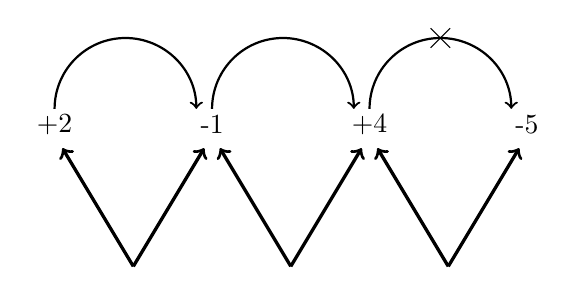
\begin{tikzpicture}[]
%\draw (-3, 0) -- (3, 0);
%\draw (0, 2.5) -- (0, -1.5);
%\draw[help lines] (-3, -1.4) grid (3, 1.4);
\draw [<-,very thick] (-2.9, .5) -- (-2, -1);
\draw [<-,very thick] (-1.1, .5) -- (-2, -1);
\draw [<-,very thick] (-.9, .5) -- (0, -1);
\draw [<-,very thick] (.9, .5) -- (0, -1);
\draw [<-,very thick] (1.1, .5) -- (2, -1);
\draw [<-,very thick] (2.9, .5) -- (2, -1);
\draw [->, thick] (-3, 1) arc [start angle = 180, end angle=0, radius=.9];
\draw [->, thick] (-1, 1) arc [start angle = 180, end angle = 0, radius=0.9];
\draw [->, thick] (1, 1) arc [start angle = 180, end angle = 0, radius=0.9];
\node [cross out, draw] at (1.9, 1.9) {};

\draw (-3, .8) node []{+2};
\draw (-1, .8) node []{-1};
\draw (1, .8) node []{+4};
\draw (3, .8) node []{-5};
\end{tikzpicture}
\end{center}

$f(-x)$ has $2$ sign changes $(+\ to\ -\ to\ +)$
\\which tells us that $f(x)$ {has no more than} $2$ negative roots 

\textbf{Obs3.} 
\end{enumerate}
\end{document}
